\chapter{Fachliche Beschreibung der Systemarchitektur}

Die vorgestellte Architektur zeigt den Aufbau einer mobilen Flutter-Applikation, die klar zwischen Frontend, Backend und
 Datenhaltung trennt. Ziel ist eine robuste, erweiterbare sowie wartungsfreundliche Lösung, die eine effiziente Kommunikation
  zwischen den Komponenten ermöglicht.

\section{Frontend (Flutter App)}
Die Flutter-App stellt die grafische Oberfläche bereit, nimmt Nutzereingaben entgegen und zeigt Inhalte wie Trainingsangebote, 
Buchungsdetails oder Suchergebnisse an. Eine vorgelagerte Service-Schicht führt REST-API-Aufrufe durch, verarbeitet eingehende
 Daten aus dem Backend und stellt über State Management einen konsistenten UI-Zustand sicher.

\section{Backend (Node.js mit Express)}
Das Backend gliedert sich in thematisch getrennte APIs:
\begin{itemize}
    \item \textbf{Auth API:} Verantwortlich für Authentifizierung, Session-Management und Zugriffsrechte.
    \item \textbf{Training API:} Stellt Endpunkte zum Abruf, Erstellen und Bearbeiten von Trainingsangeboten bereit.
    \item \textbf{Booking API:} Ermöglicht das Reservieren, Stornieren und Verwalten von Buchungen.
    \item \textbf{Search API:} Unterstützt Suche und Filterung von Trainingsangeboten.
\end{itemize}
Der Express-Server dient als zentrale Kommunikationsschnittstelle, leitet Requests an die richtigen API-Routen weiter,
 koordiniert Datenbankzugriffe und steuert bei Bedarf weitere Dienste (z. B. E-Mail-Versand).

\section{Datenbank (MySQL)}
Eine MySQL-Datenbank, angebunden über einen Connection Pool, stellt performante, relationale Datenstrukturen bereit. Wichtige
Entitäten sind:
\begin{itemize}
    \item \textbf{Users:} Nutzerprofile und Logininformationen
    \item \textbf{Trainings:} Trainingsangebote mit Titeln, Beschreibungen, Terminen und Dozenten
    \item \textbf{Bookings:} Buchungsdaten zu einzelnen Nutzern und Kursen
    \item \textbf{Tags:} Zur thematischen Kategorisierung von Angeboten
\end{itemize}

\section{E-Mail-Service (SMTP-Server)}
Automatisierte Nachrichten wie Buchungsbestätigungen oder Passwort-Resets werden über einen SMTP-Server versendet.

\section{Zusammenfassung}
Das Gesamtsystem trennt UI (Flutter) von Logik (Node.js-Backend) und Datenhaltung (MySQL), integriert definierte REST-APIs
und nutzt einen E-Mail-Service für Benachrichtigungen. Diese Aufteilung gewährleistet Flexibilität, Skalierbarkeit und
erleichtert Wartung sowie Weiterentwicklung.

\chapter{Umfassende fachliche Beschreibung des gezeigten Sequenzdiagramms}
Das Sequenzdiagramm zeigt die zeitliche Abfolge konkreter Interaktionen zwischen Flutter-App, Node.js-API, MySQL-Datenbank und
 E-Mail-Service. Es verdeutlicht die Prozessschritte bei Authentifizierung, Trainingsverwaltung, Buchungen sowie Termin- und 
 Pausenplanung. Statt der allgemeinen statischen Architektur veranschaulicht es, wie einzelne Funktionen operativ zusammenspielen.

\section{Allgemeiner Zweck}
Das Sequenzdiagramm dient dazu, den Fluss von Anfragen und Antworten in chronologischer Reihenfolge darzustellen. Vertikale 
Linien repräsentieren beteiligte Komponenten, horizontale Pfeile deren Kommunikation. Es zeigt, welche Daten wann angefragt, 
geprüft und zurückgeliefert werden. So entsteht ein tieferes Verständnis dafür, wie scheinbar einfache Nutzeraktionen komplexe
 interne Abläufe auslösen.

\section{Beispiel: Authentifizierung}
Ein Login-Request der Flutter-App an die Node.js-API führt zu einer Datenbankabfrage zur Verifizierung. Bei korrekten Credentials
 wird ein JWT-Token erzeugt und an die App zurückgesendet. Das Diagramm macht transparent, dass ein einzelner Login-Vorgang aus 
 mehreren Teilschritten besteht: Eingabe prüfen, Datenbankanfrage, Token generieren, Antwort zurückgeben.

\section{Training Management}
Anfragen wie \texttt{GET /api/trainings} liefern strukturierte Listen verfügbarer Kurse. Hierdurch wird klar, dass die Node.js-API 
nicht einfach Daten durchreicht, sondern diese gezielt aus verschiedenen Tabellen aggregiert. Beim Erstellen neuer Trainings über einen \texttt{POST}-Request validiert die API eingehende Daten, legt neue Einträge in der Datenbank an und bestätigt den Erfolg. Ähnliches gilt für komplexere Funktionen wie die Suche nach Trainings (\texttt{GET /api/trainings/search}), wo Eingabefilter übernommen, passende Datensätze gefiltert und resultierende Listen zurückgegeben werden. Teilweise starten diese Abläufe nachgelagerte Prozesse, z. B. das Versenden von Benachrichtigungen über den E-Mail-Service, um andere Stakeholder auf neue Trainings hinzuweisen.

\section{Booking Management}
Beim Buchen von Terminen sind Zustandsabfragen entscheidend. Eine Buchungsanfrage (\texttt{POST /api/bookings}) prüft zunächst Verfügbarkeiten und Kontingente. Sind Kapazitäten vorhanden, wird ein neuer Datensatz eingetragen, der Erfolg bestätigt und bei Bedarf eine Bestätigungs-E-Mail versendet. Das Sequenzdiagramm verdeutlicht so die interne Logik: Datenvalidierung, Aktualisierung von Verfügbarkeiten und Rückmeldung an den Nutzer geschehen in koordinierter Reihenfolge.

\section{Termin- und Pausenplanung (Schedule Management)}
Funktionen zur Verwaltung von Terminen und Pausen demonstrieren, wie zeitliche Strukturen abgebildet werden. \texttt{GET}-Requests liefern Terminübersichten, \texttt{POST}-Requests legen neue Pausen fest. Auch hier durchläuft die Anfrage eine Kette von Überprüfungen und Datenbankoperationen, bevor die App entsprechende Informationen zurückerhält. Das Diagramm zeigt, wie diese technischen Schritte zusammenwirken, um letztlich eine nutzerfreundliche Terminübersicht bereitzustellen.

\section{Besonderheiten}
Das Sequenzdiagramm verdeutlicht, dass die API nicht nur reine Vermittlungsschicht ist, sondern aktiv Logik einbringt: Validierung von Eingaben, Datenverknüpfungen, Prüfung von Geschäftsregeln und Zuständen. Die Integration des E-Mail-Services macht zudem deutlich, dass externe Dienste nahtlos eingebunden sind.

Insgesamt liefert das Sequenzdiagramm einen praxisnahen Einblick in die interne Funktionsweise. Wer es betrachtet, versteht besser, wie aus simplen Nutzeraktionen – wie etwa „Login“ oder „Kurs buchen“ – komplexe Abfolgen von Datenbankabfragen, Logik und Kommunikationsschritten entstehen. So wird nachvollziehbar, wo potenzielle Fehlerquellen liegen, wie Änderungen an einer Stelle Auswirkungen auf andere Bereiche haben und welche Rolle externe Systeme spielen.

\chapter{Umfassende Beschreibung der Datenbankstruktur}
Das Datenmodell bildet die fachliche Grundlage des Systems, indem es Schulungsangebote, ihre zeitliche Struktur, Buchungen, Kategorisierungen (Tags), Dozenten sowie Nutzende klar abbildet. Die Datenbank verfolgt einen relationalen Ansatz, bei dem Primär- und Fremdschlüsselbeziehungen komplexe Szenarien unterstützten.

\section{Zentrale Entität: Schulungen}
Die Tabelle \texttt{schulungen} stellt einzelne Trainings oder Kurse dar. Neben \texttt{id} und \texttt{titel} finden sich Felder für \texttt{beschreibung}, \texttt{ort}, \texttt{gesamt\_start-} und \texttt{enddatum}, \texttt{max\_teilnehmer} sowie Verweise auf den verantwortlichen Dozenten. Diese Entität ist der inhaltliche Kern, um den sich weitere Tabellen gruppieren.

\section{Zeitliche Struktur: schulung\_sessions, schulung\_pause, schulungstermin, schulungstermin\_zeitabschnitt}
Mehrtägige oder mehrmodulige Kurse lassen sich mit \texttt{schulung\_sessions} in einzelne Zeiteinheiten aufschlüsseln. Jede Session hat Datum, Start- und Endzeiten, um den Kurs planbar und transparent zu machen. Pausen werden in \texttt{schulung\_pause} festgehalten und verhindern etwaige Buchungen in den unterbrochenen Zeiträumen. Termine (\texttt{schulungstermin}) und feinere zeitliche Abschnitte (\texttt{schulungstermin\_zeitabschnitt}) erlauben es, noch detailliertere Zeitpläne abzubilden. So entsteht eine fein granulare Modellierung von Kursstrukturen, Zeitfenstern und Pausen.

\section{Tagging: tags und schulungen\_tags}
Die Tag-Tabellen ermöglichen eine flexible Kategorisierung von Schulungen. Tags können etwa thematische Stichworte oder Schwierigkeitsgrade umfassen. Durch die n:m-Beziehung in \texttt{schulungen\_tags} lassen sich Schulungen mit beliebig vielen Tags assoziieren, was dynamische Filterungen und Suchoptionen unterstützt.

\section{Dozenten und Users}
Die \texttt{dozenten}-Tabelle erfasst Lehrpersonal mit Kontaktdaten und Fachgebieten. Über \texttt{dozent\_id} in \texttt{schulungen} wird eine klare Zuordnung hergestellt. Die \texttt{users}-Tabelle bildet die Endnutzenden ab – Teilnehmende, Administratoren oder weitere Rollen. Hier sind Login





\begin{figure}[p]
    \centering
    \rotatebox{90}{%
        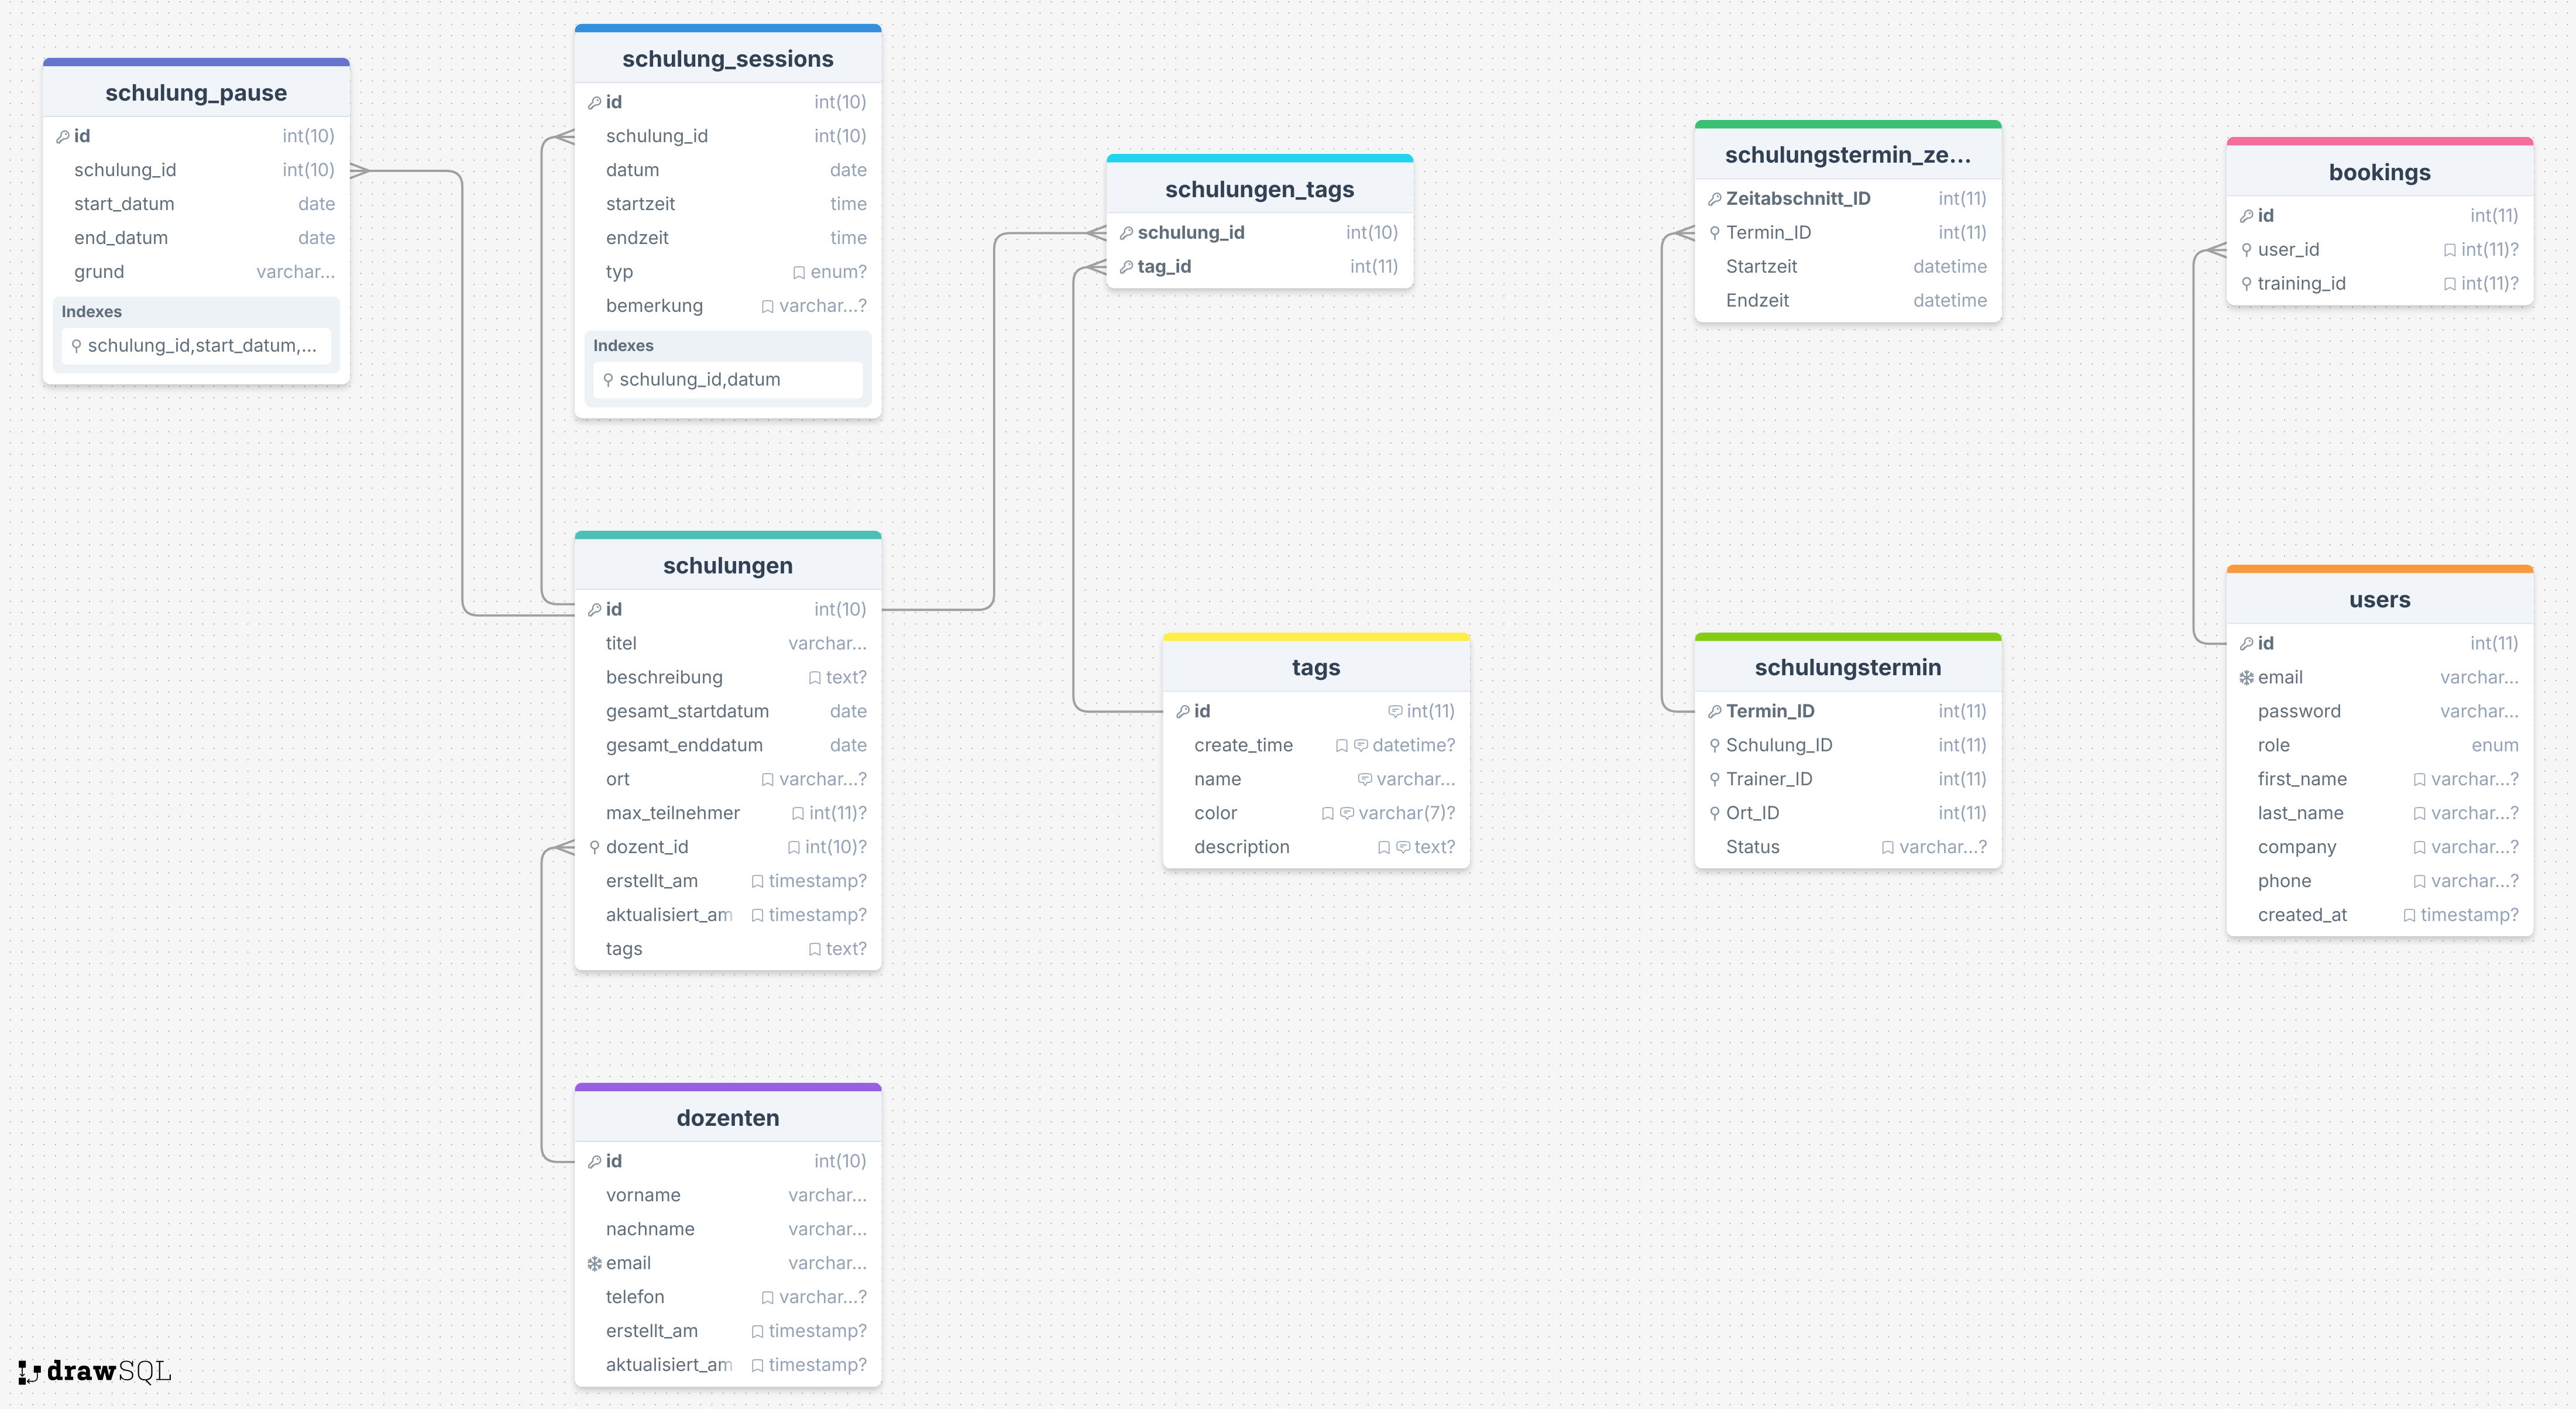
\includegraphics[width=\textheight]{img/MariaDB.png}%
    }
    \caption{Informationen zu den Trainings}
    \label{MAriaDB}
\end{figure}

\begin{figure}[p]
    \centering
    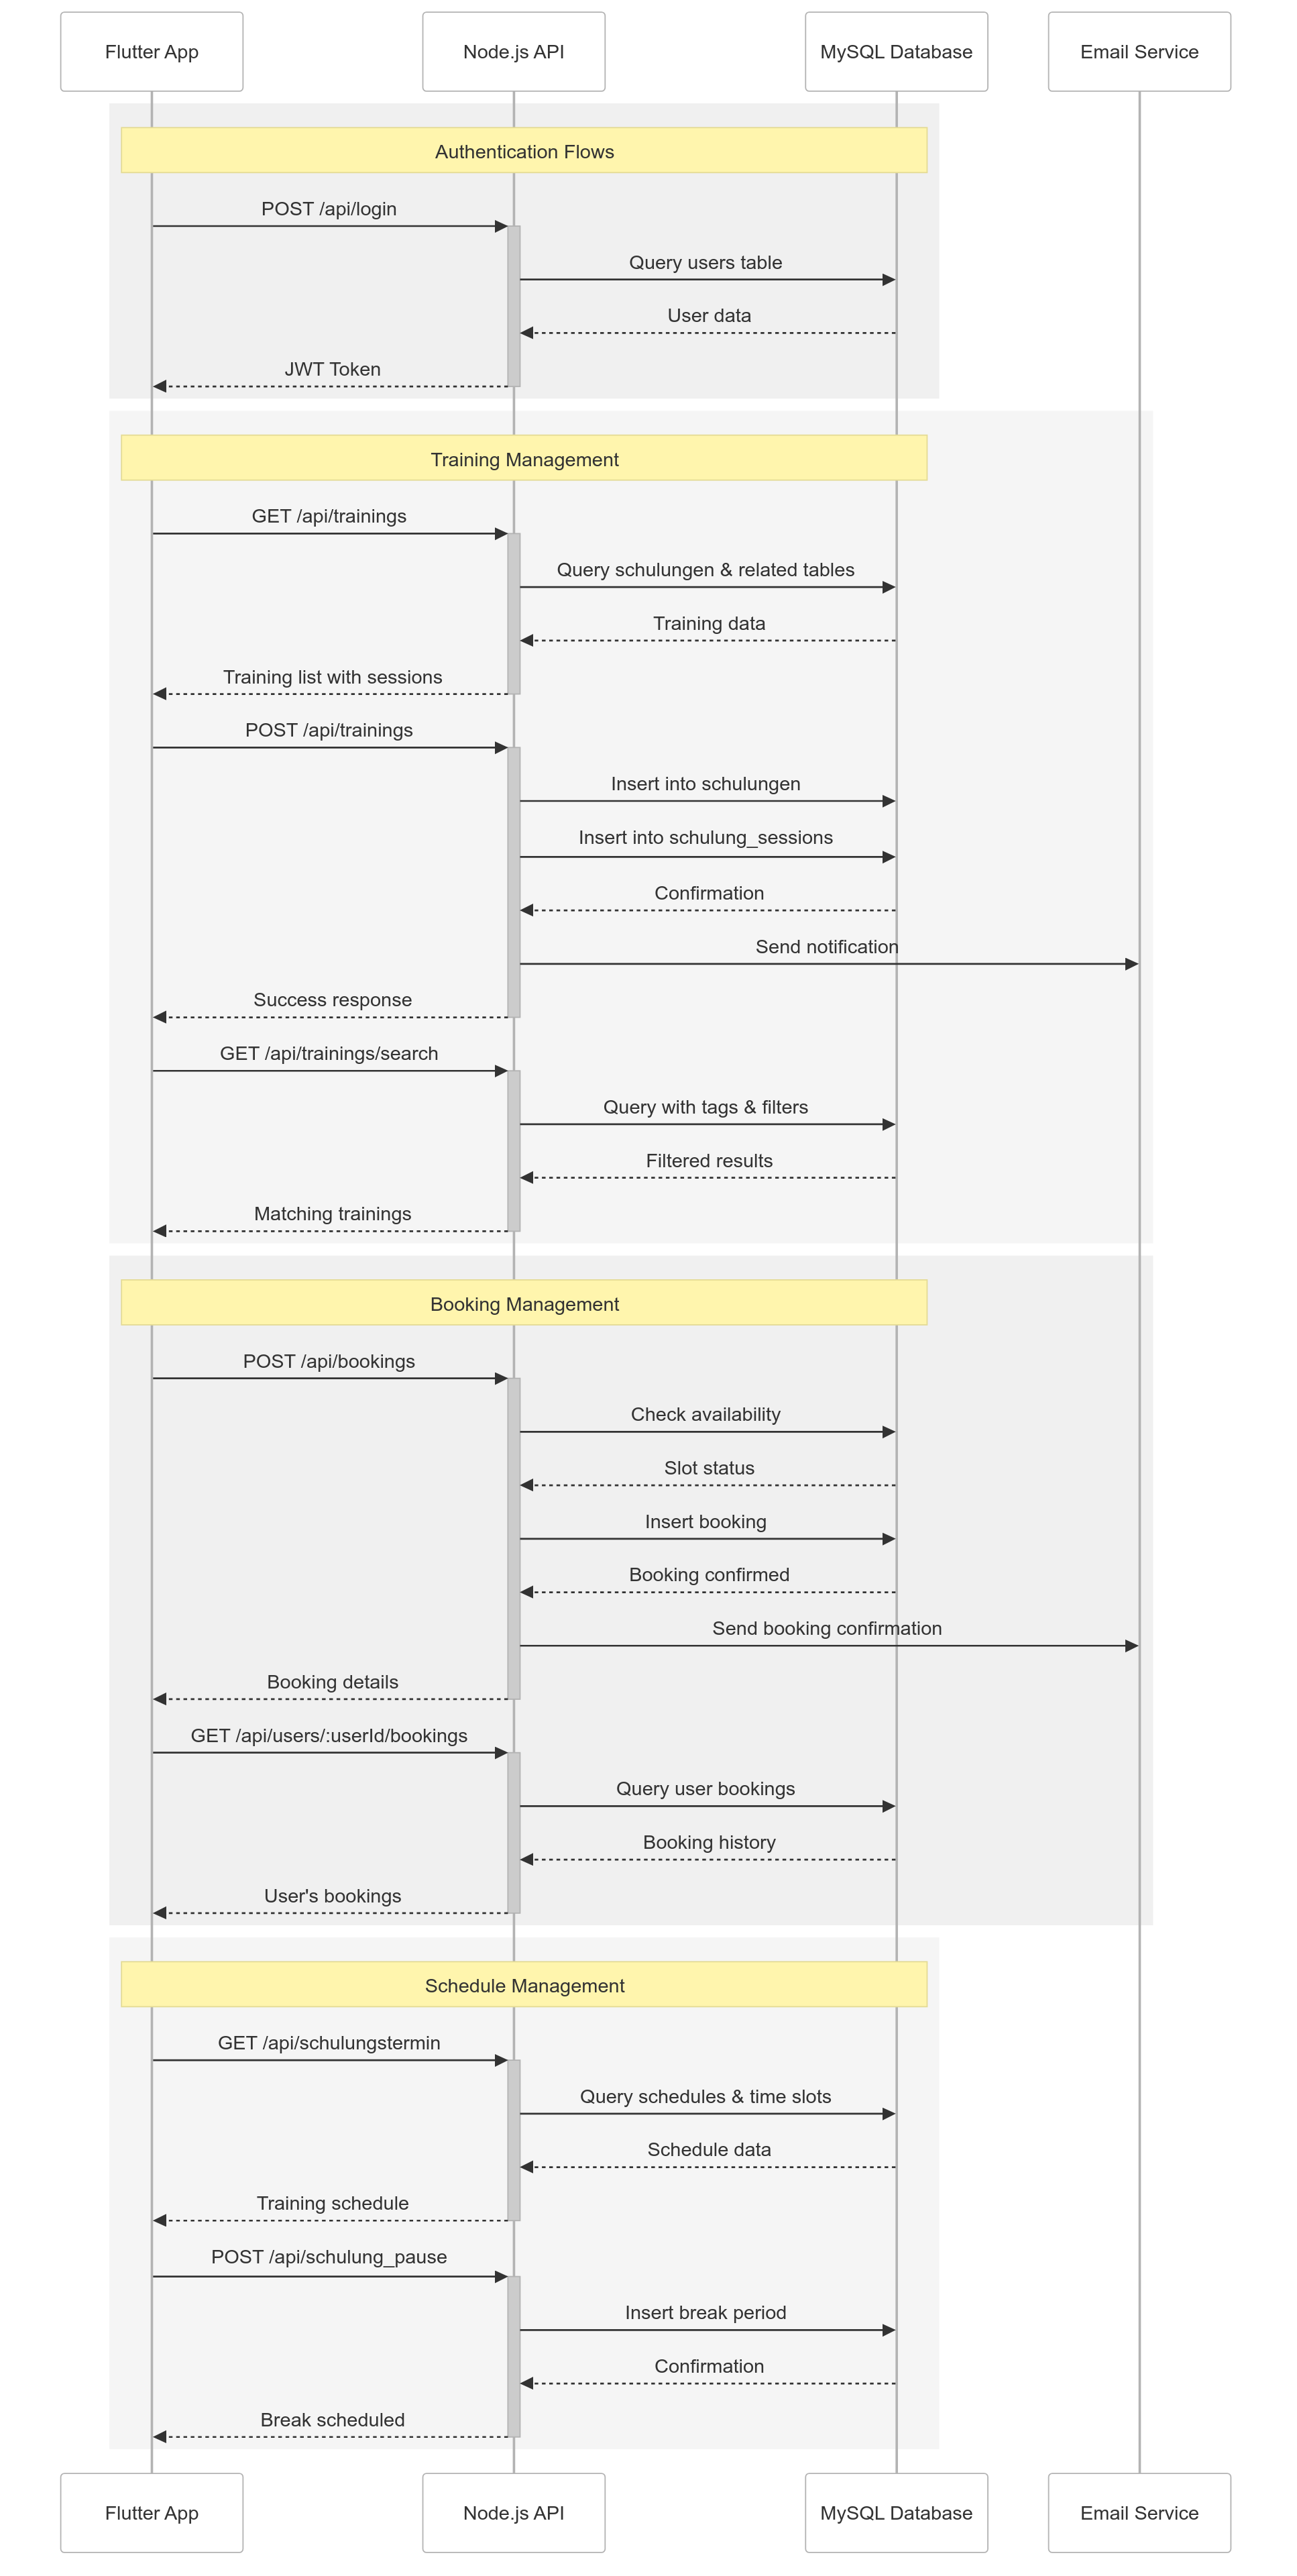
\includegraphics[width=\textwidth, height=\textheight, keepaspectratio]{img/Ablaufdiagram.png}%
    \caption{Ablaufsdiagramm}
    \label{Ablaufsdiagramm}
\end{figure}


\begin{figure}[p]
    \centering
    \rotatebox{90}{%
        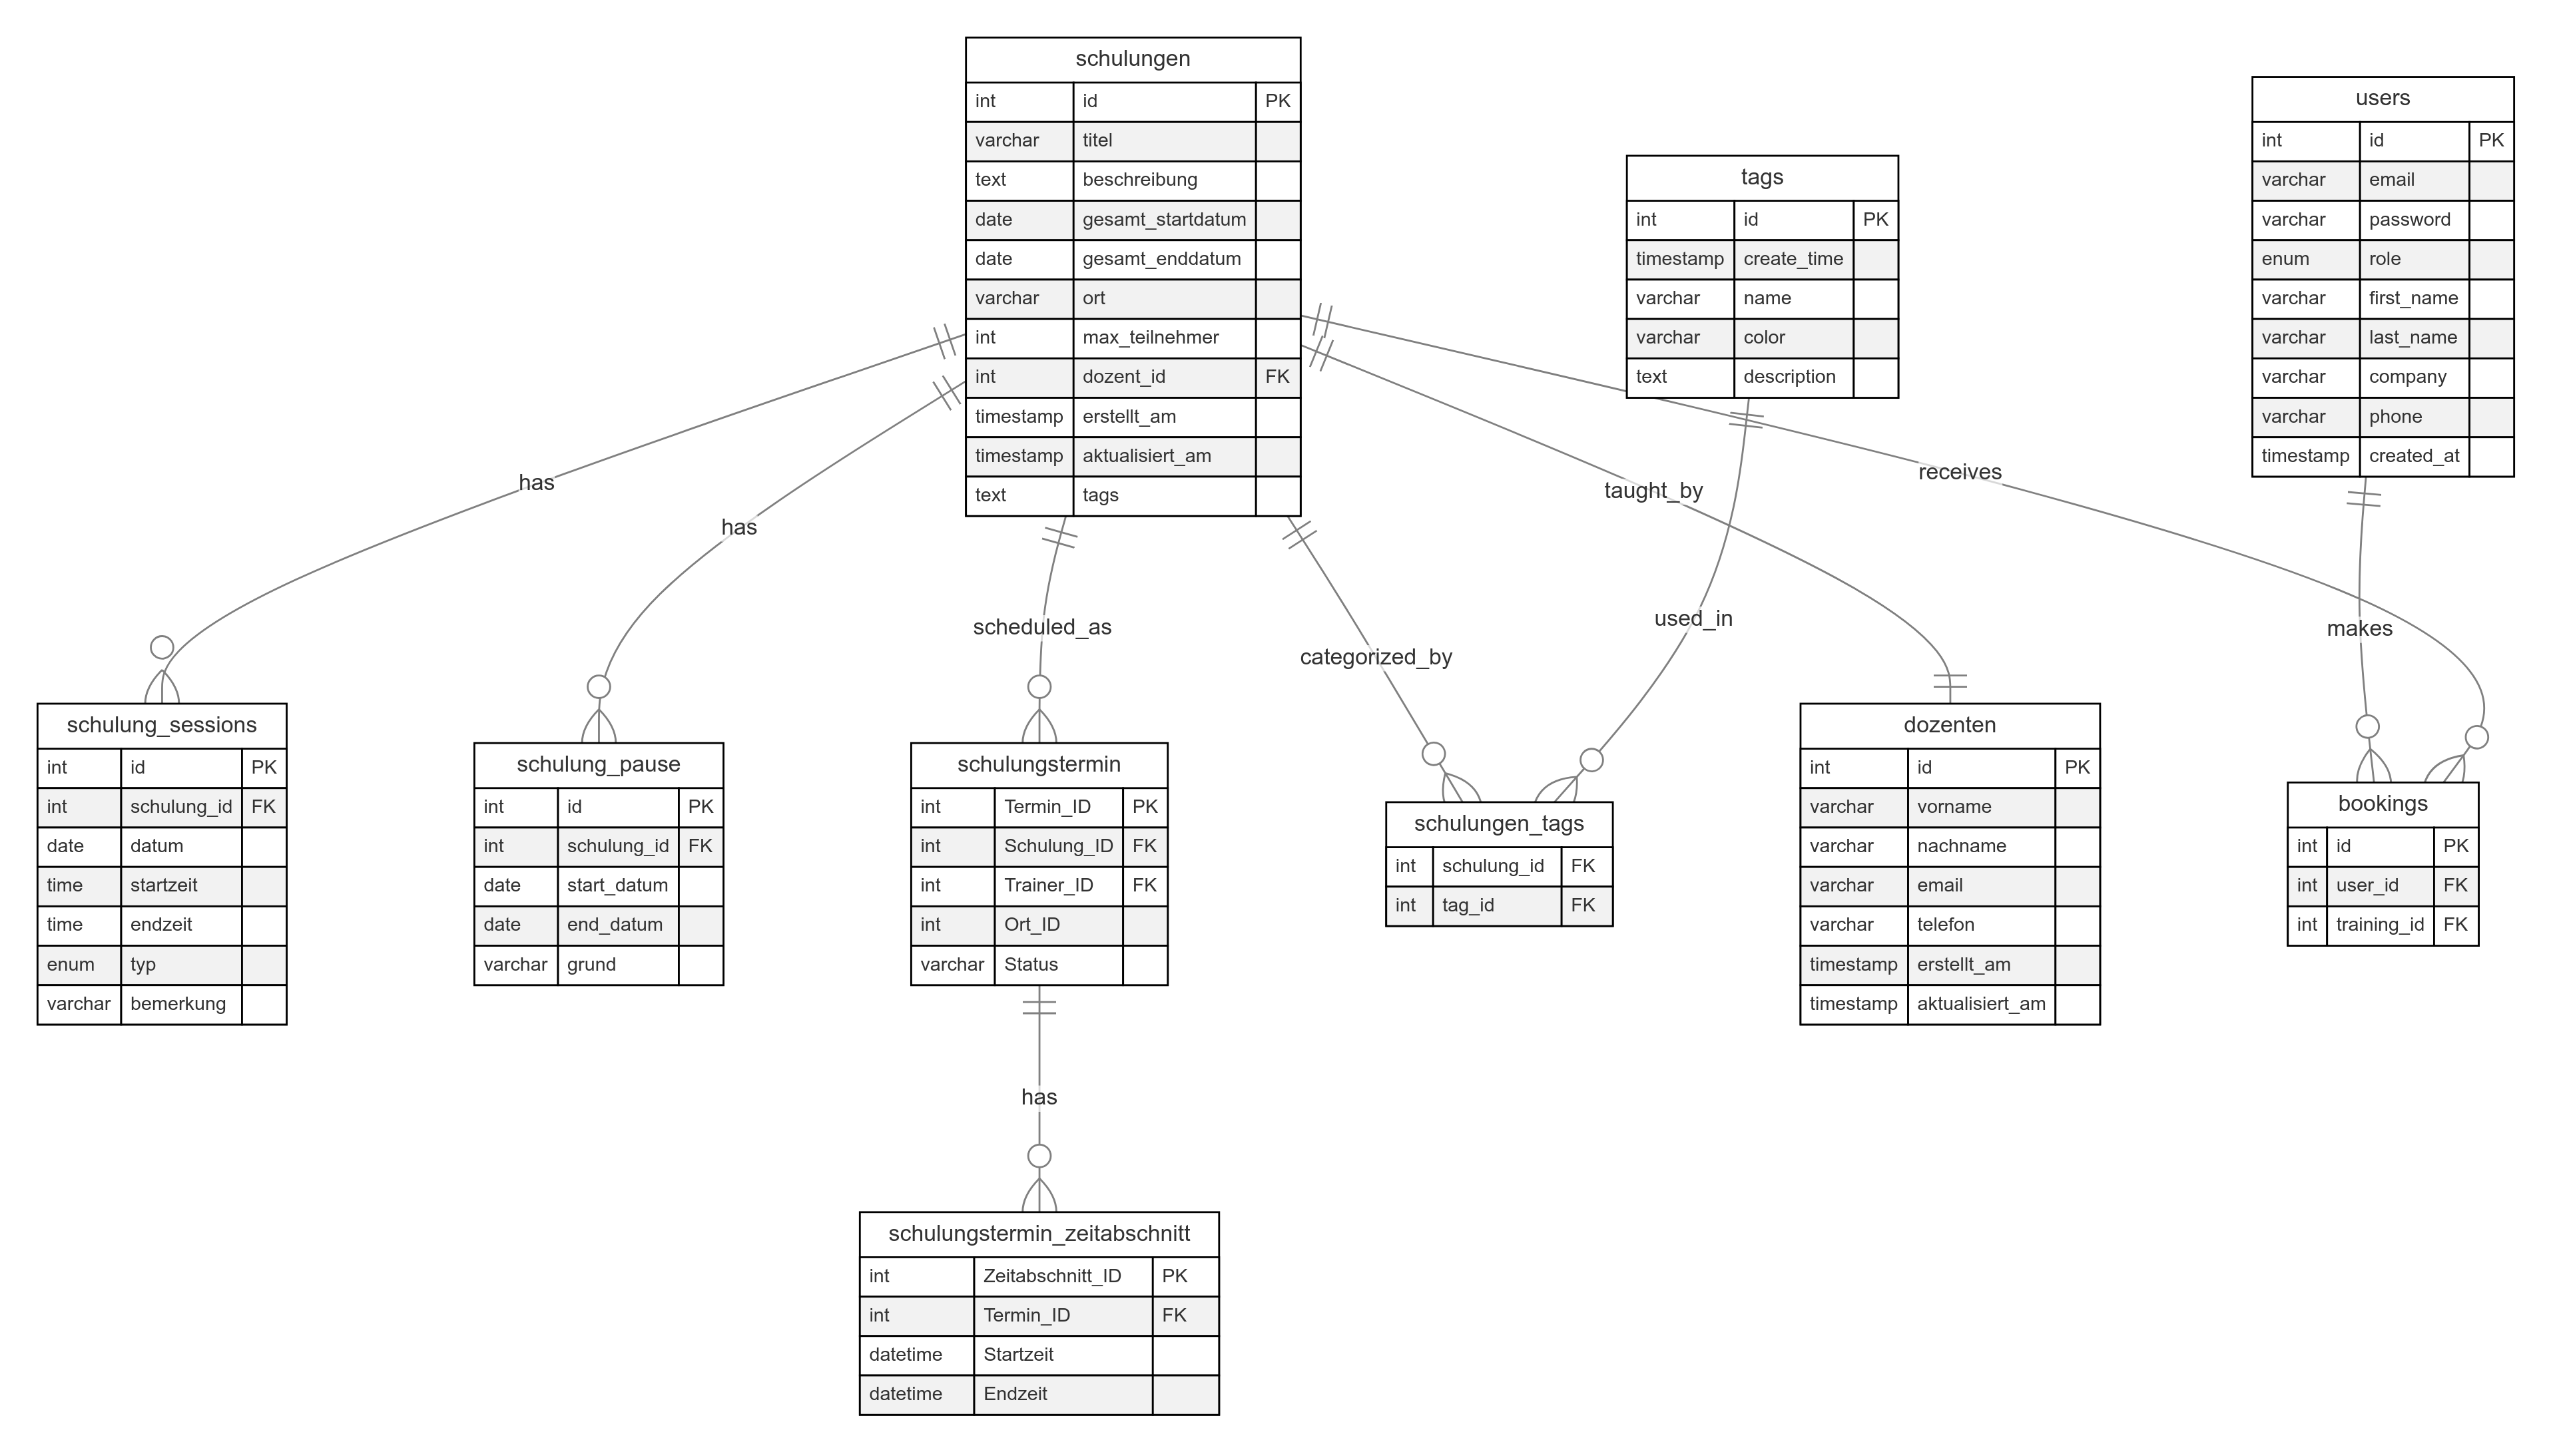
\includegraphics[width=\textheight]{img/Datenbankstruktur.png}%
    }
    \caption{Datenbankstruktur}
    \label{Datenbankstruktur}
\end{figure}

\begin{figure}[p]
    \centering
    \rotatebox{90}{%
        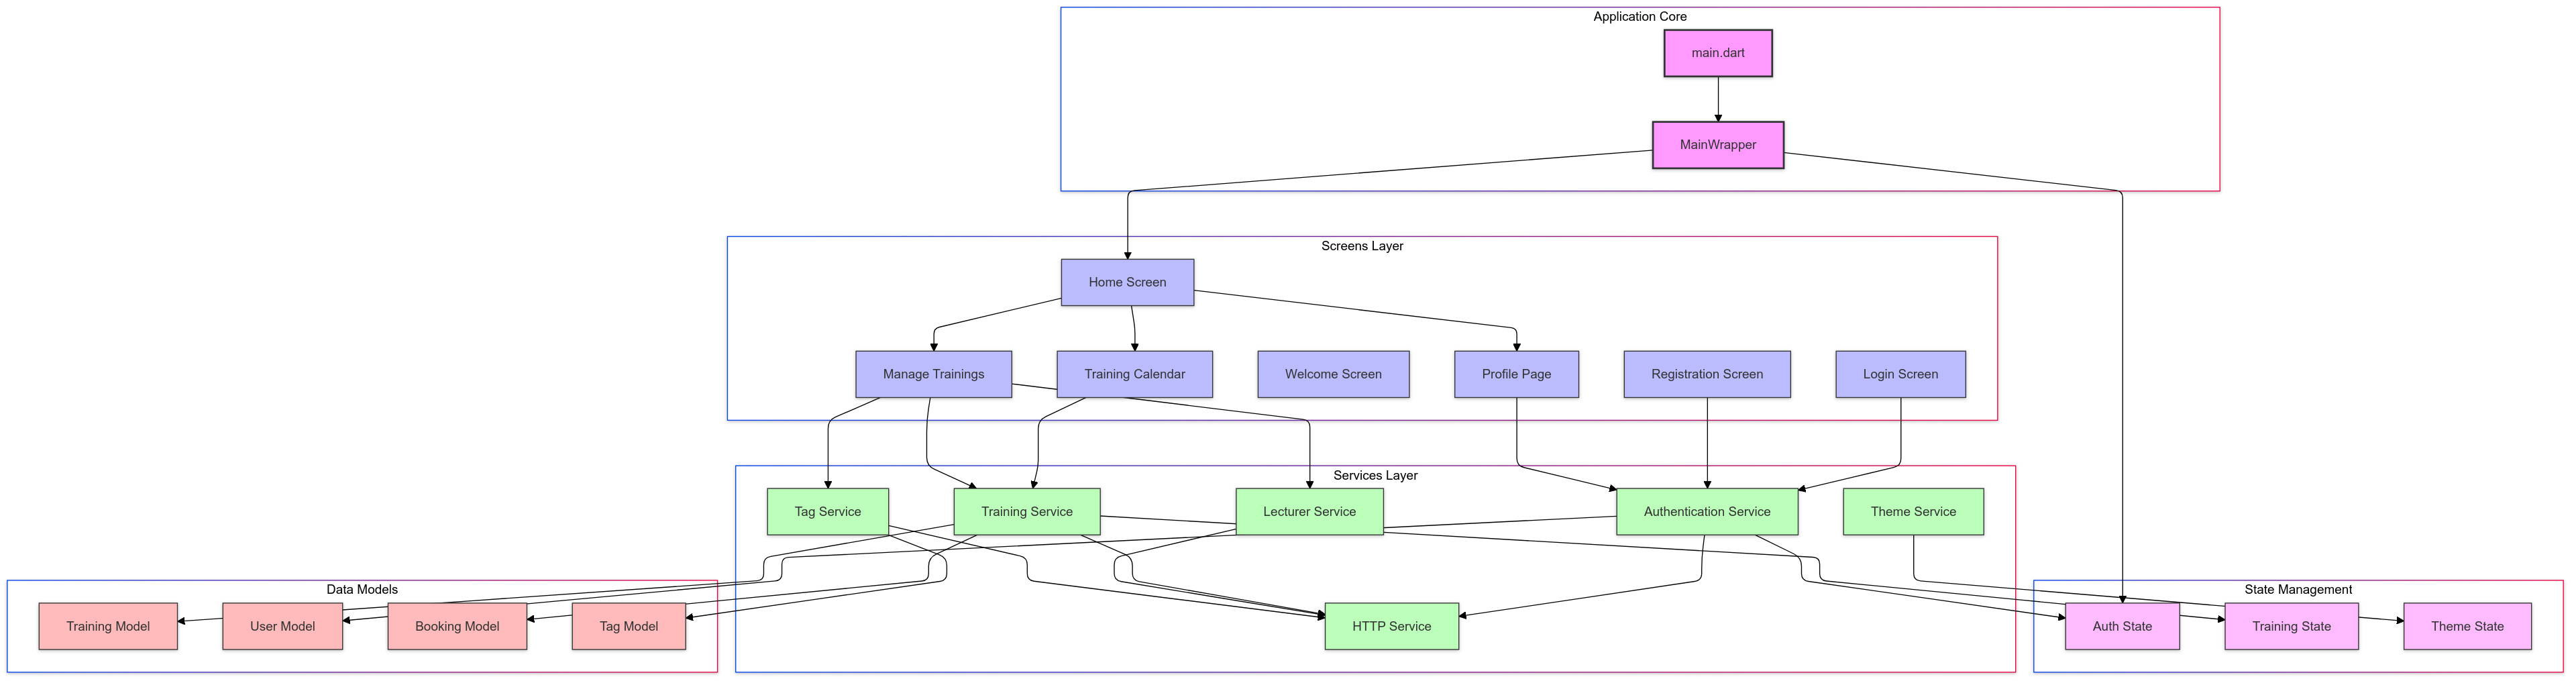
\includegraphics[width=\textheight]{img/Component_Diagram.png}%
    }
    \caption{Compnent Diagramm}
    \label{Compnent Diagramm}
\end{figure}



